\documentclass[12pt,letterpaper]{hmcpset}
\usepackage[margin=1in]{geometry}
\usepackage{graphicx}
\usepackage{amsmath}
\usepackage{tikz}
\usepackage{pdfpages}
\usepackage{xcolor}


% info for header block in upper right hand corner
\name{---}
\class{Physics 24a}
\assignment{Forces and Equations of Motion}
\duedate{Monday, January 25, 2016}

\newcommand{\dg}[1]{#1^o}

% set numbering style for enumerated lists to be of form (a), (b), (c), etc.
\renewcommand{\labelenumi}{{(\alph{enumi})}}

% command to make 1.5in wide image centered on page
\newcommand{\diagram}[1]{\begin{center}\includegraphics[width=1.5in]{#1}\end{center}}

\begin{document}

\problemlist{3.\{5, 12, 17, 22, 25\}}

% 3.5 %
\begin{problem}[1 - Mass and Axle* - 3.5]
    A mass $m$ is connected to a vertical revolving
    axle by two strings of length $l$, each making
    an angle of $\dg{45}$ with the axle, as shown.
    Both the axle and mass are revolving with angular 
    velocity $\omega$. Gravity is directed downward.

    \begin{enumerate}
        \item Draw a clear force diagram for $m$.
        \item Find the tension in the upper string,
            $T_{\text{up}}$, and the lower string 
            $T_{\text{low}}$.
    \end{enumerate}

    \begin{center}
    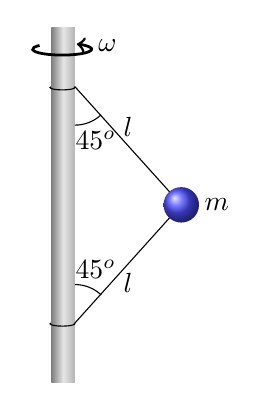
\begin{tikzpicture}[scale=0.75]
      % attempt to draw three-d rod
      \shade[left color=black!50, right color=black!30, middle color=black!10]  (-0.2,3) rectangle
      (0.2,-3);
      \draw[line width=1,->] (-0.4,2.7) arc[start angle=140,delta angle=280, x
      radius = 0.5, y radius = 0.1];
      \node at (0.75,2.7) {$\omega$};
      % upper string
      \draw (-0.21,2) arc[x radius=0.21, y radius=0.04, start angle=160,
      end angle=380];
      \draw (-0.21,-2) arc[x radius=0.21, y radius=0.04, start angle=160,
      end angle=380];
      \draw (0.2,-2) --node[below]{$l$} (2,0) --node[above]{$l$} (0.2,2);
      \shade[ball color=blue!70] (2,0) circle[radius=0.3];
      \node at (2.6,0){$m$};
      % arcs
      \draw (0.2,-2+0.65) arc(90:47:0.65);
      \node at (0.55,-1.1){$\dg{45}$};
      \draw (0.2,2-0.65) arc (-90:-47:0.65);
      \node at (0.55,1.1){$\dg{45}$};  
    \end{tikzpicture}
    \end{center}
\end{problem}

\begin{solution}
    \vfill
\end{solution}
\newpage


% 3.12 %
\begin{problem}[2 - Capstan - KK 3.12]
    A device called a capstan is used
    aboard ships in order to control a rope
    which is under great tension. The rope
    is wrapped around a fixed drum, usually
    for several turns (the drawing shows 
    about a three-quarter turn). The load on
    the rope pulls it with a force $T_{A}$, 
    and the sailor holds it with a much smaller
    force $T_{B}$. Show that $T_{B} = T_{A}e^{-\mu\theta}$,
    where $\mu$ is the coefficient of static friction
    and $\theta$ is the total angle subtended
    by the rope on the drum.

    \begin{center}
    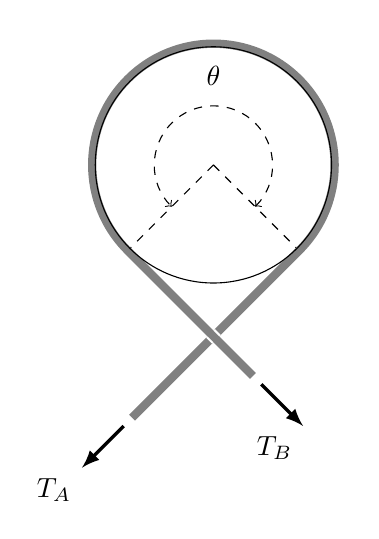
\begin{tikzpicture}[scale=0.75]
        \def\rad{2cm}
        \draw[dashed] (0,0) -- (-45:\rad) 
                      (0,0) -- (-135:\rad);
        \draw[dashed, <->] (-45:\rad/2) arc(-45:225:\rad/2);
        \node at (0,0.75*\rad){$\theta$};
        % now the rope 
        \draw[gray,line width=3] (-45:\rad+1.5pt) -- ++(-135:4)
          (-45:\rad+1.5pt) arc(-45:225:\rad+1.5pt) -- ++(-45:3);
        \begin{scope}[shift={(-45:\rad+1.5pt)}]
            \draw[-latex, very thick] (-135:4.2) -- ++(-135:1) node[anchor=north east]{$T_{A}$};
        \end{scope}
        \begin{scope}[shift={(-135:\rad+1.5pt)}]
            \draw[-latex, very thick] (-45:3.2) -- ++(-45:1) node[anchor=north east]{$T_{B}$};
        \end{scope}
        \begin{scope}[shift={(-135:\rad)}, rotate=-45]
            \fill[fill=white] (\rad-0.5pt,0.5pt) rectangle ++(4pt,1pt);
            \fill[fill=white] (\rad-0.5pt,-3.5pt) rectangle ++(4pt,-1pt);
        \end{scope}
        \draw (0,0) circle[radius=\rad];
    \end{tikzpicture}
    \end{center}
\end{problem}

\begin{solution}
    \vfill
\end{solution}
\newpage

% 3.17 %
\begin{problem}[3 - Turning car* - KK 3.17]
    A car enters a turn whose radius is $R$.
    The road is banked at angle $\theta$, and
    the coefficient of friction between the
    wheels and the road is $\mu$. Find the 
    maximum and minimum speeds for the car to 
    stay on the road without skidding sideways.

    \diagram{img/3_17.png}
\end{problem}

\begin{solution}
    \vfill
\end{solution}
\newpage

% 3.22 %
\begin{problem}[4 - Mass, string, and ring* - KK 3.22]
    A mass $m$ whirls around on a string
    which passes through a ring, as shown.
    Neglect gravity. Initially the mass
    is distance $r_{0}$ from the center and 
    is revolving at angular velocity $\omega_{0}$. 
    The string is pulled with constant velocity
    $V$ starting at $t = 0$ so that the radial 
    distance to the mass decreases. Draw a force
    diagram and obtain a differential equation for
    $\omega$. This equation is quite simple and 
    can be solved either by inspection
    or by formal integration. Find

    \begin{enumerate}
    \item $\omega(t)$.
    \item The force needed to pull the string.
    \end{enumerate}

    \diagram{img/3_22.png}
\end{problem}

\begin{solution}
    \vfill
\end{solution}
\newpage

% 3.25 %
\begin{problem}[5 - Hovercraft - KK 3.25]
The Eureka Hovercraft Corporation wanted
to hold hovercraft races as an advertising 
stunt. The hovercraft supports itself 
by blowing air downward, and has a big 
fixed propeller on the top deck for forward
propulsion. Unfortunately, it has no 
steering equipment, so the pilots found that 
making high speed turns was very difficult.
The company decided to overcome this problem 
by designing a bowl-shaped track in which the
hovercraft, once up to speed, would coast 
along in a circular path with no need to steer.

When the company held their first race, they 
found to their dismay that the craft took 
exactly the same time $T$ to circle the track,
no matter what its speed. Find the equation
for the cross-section of the bowl in terms of $T$.
\end{problem}

\begin{solution}
    \vfill
\end{solution}
\newpage

\end{document}
